% Created 2022-03-17 Thu 20:15
% Intended LaTeX compiler: pdflatex
\documentclass[11pt]{article}
\usepackage[utf8]{inputenc}
\usepackage[T1]{fontenc}
\usepackage{graphicx}
\usepackage{grffile}
\usepackage{longtable}
\usepackage{wrapfig}
\usepackage{rotating}
\usepackage[normalem]{ulem}
\usepackage{amsmath}
\usepackage{textcomp}
\usepackage{amssymb}
\usepackage{capt-of}
\usepackage{hyperref}
\usepackage{minted}
\date{\today}
\title{}
\hypersetup{
 pdfauthor={},
 pdftitle={},
 pdfkeywords={},
 pdfsubject={},
 pdfcreator={Emacs 27.2 (Org mode 9.4.4)}, 
 pdflang={English}}
\begin{document}

\tableofcontents

\section{STEADY DIFFUSION EQUATIONS}
\label{sec:org8305b59}
\subsection{Problem Definition}
\label{sec:orgf1d1e6f}
We consider the solution of a \uline{steady}, \uline{1D} heat diffusion equation
\begin{equation}
-k \nabla^2 T - S = 0
\end{equation}
\subsection{Discretization}
\label{sec:org4a9bc86}
Recall our diffusion term can be discretized as:
\begin{equation}
\int_S \textbf{J} \cdot \textbf{n} dS \approx \sum_{i=0}^{N_{ip}-1} \textbf{J}_{ip}\cdot \textbf{n}_{ip}A_{ip}
\end{equation}
Our flux \(\textbf{J}\) here is the \uline{diffusive} flux, so: \(\textbf{J} = -k \nabla T\). Thus:
\begin{equation}
\int_S \textbf{J} \cdot \textbf{n} dS \approx -\sum_{i=0}^{N_{ip}-1} k_{ip} \nabla T_{ip}  \cdot \textbf{n}_{ip}A_{ip}
\end{equation}
We assume constant thermal conductivity, \(k_{ip} = k\). A 1D control volume, with West/East faces and unit vectors drawn, is shown below:
\begin{center}
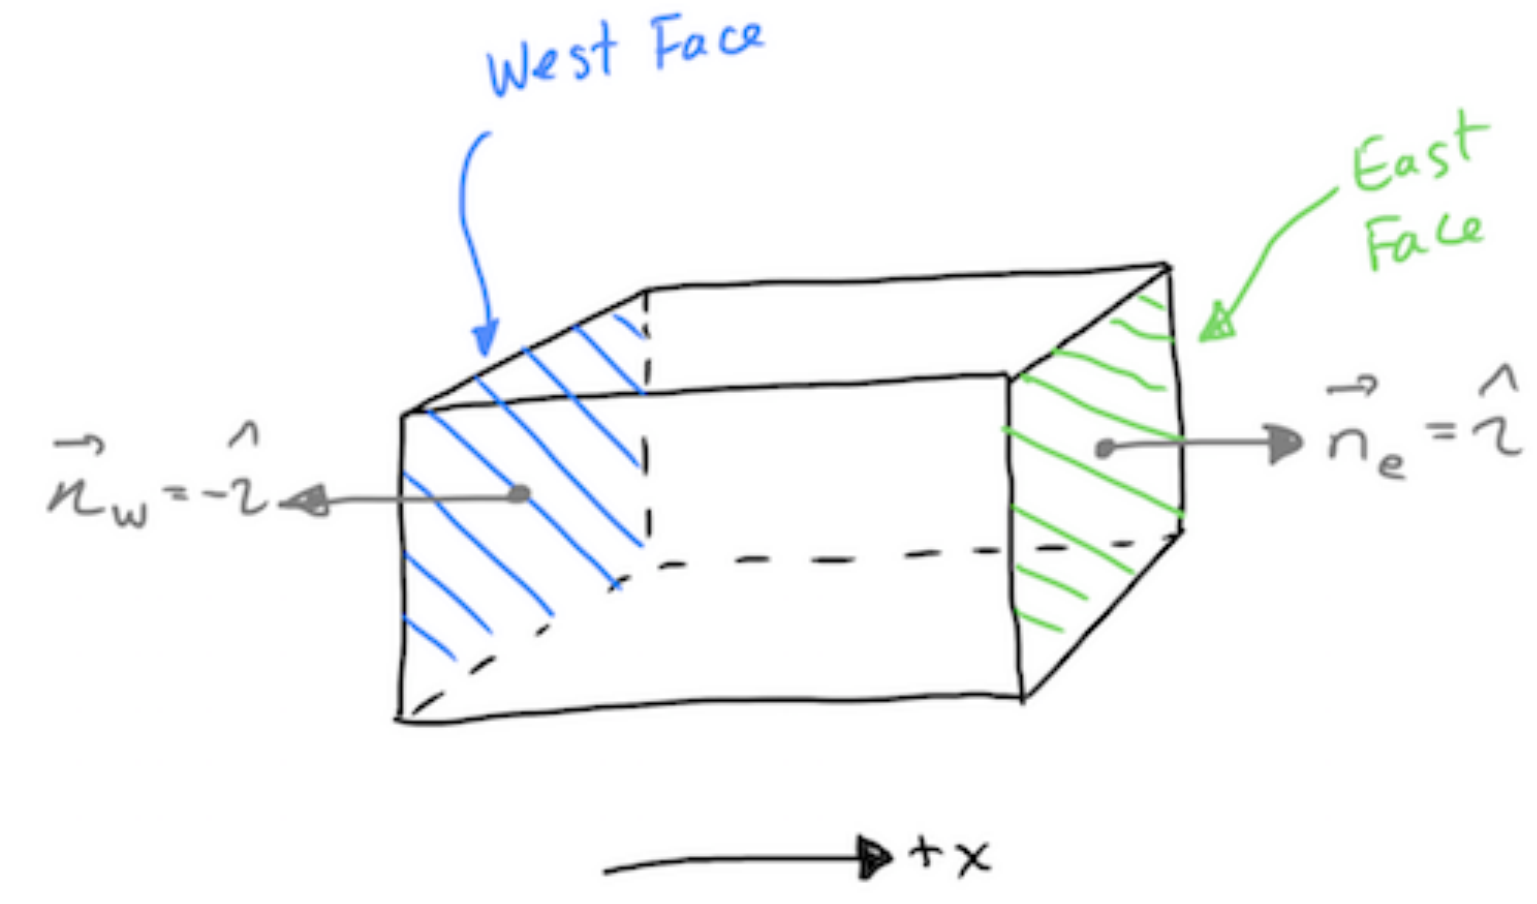
\includegraphics[scale=0.2]{pic/heat1D_CV.png}
\end{center}
Since we are in 1D, our unit vector is in the \(\textbf{i}\) only.\\
Thus, \(\nabla T \cdot \textbf{n} = \nabla T \cdot \textbf{i}\).\\
But, \(\nabla T \cdot \textbf{i} = \left < \frac{\partial T}{\partial x} \textbf{i} + \frac{\partial T}{\partial y} \textbf{j} + \frac{\partial T}{\partial z} \textbf{k}
  \right > \cdot \left <1 \textbf{i} + 0 \textbf{j} + 0 \textbf{k}    \right> = \frac{\partial T}{\partial x}\). \\
With these points in mind, the discretization for the diffusion term is simplified to:
\begin{equation}
\int_S \textbf{J} \cdot \textbf{n} dS \approx k \left .\frac{\partial T}{\partial x}\right|_w A_w
- k \left .\frac{\partial T}{\partial x}\right|_e A_e 
\end{equation}
The diagram below shows the cell locations and the nomenclature for the distance between them, note how \(\Delta x\) is center-center
\begin{center}
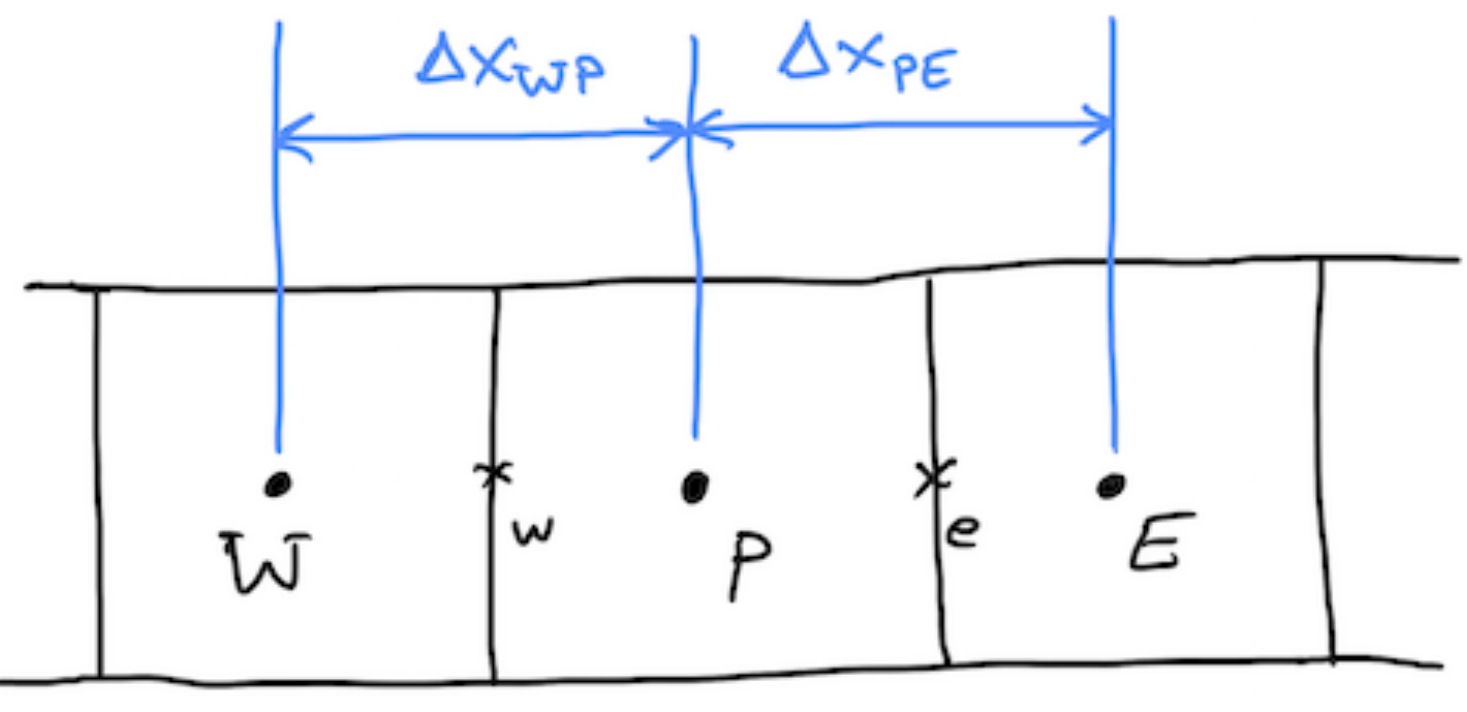
\includegraphics[scale=0.2]{pic/heat1D_cell.png}
\end{center}
We apply \uline{finite differences} to the derivatives in the diffusion term, i.e.:
\begin{equation}
k \left .\frac{\partial T}{\partial x}\right|_w A_w - k \left .\frac{\partial T}{\partial x}\right|_e A_e
= k\frac{T_P-T_W}{\Delta x_{WP}}A_w - k\frac{T_E-T_P}{\Delta x_{PE}}A_e
\end{equation}
Our discretized source term is simply:
\begin{equation}
\int_V SdV \approx S_PV_P
\end{equation}
where \(S_P\) = value of source term \textbf{within} the cell, and \(V_P\) = cell volume.\\
Put everything on one side, we can form the \uline{residual equation} for the cell \(\textbf{P}\) as:
\begin{equation}
r_P = - k\frac{T_E-T_P}{\Delta x_{PE}}A_e + k\frac{T_P-T_W}{\Delta x_{WP}}A_w - S_PV_P
\end{equation}
or expressing in terms of the diffusive fluxes, \(\textbf{F}^d\), through each face:
\begin{equation}
r_P = F_{e}^d - F_{w}^d - S_PV_P
\end{equation}
where:\\
\begin{alignat}{2}
F_{e}^d &= - k\frac{T_E-T_P}{\Delta x_{PE}}A_e &&= -D_e(T_E- T_P)\\
F_{w}^d &= - k\frac{T_P-T_W}{\Delta x_{WP}}A_w &&= -D_w(T_P- T_W)\\
D_e &= \frac{kA_e}{\Delta x_{PE}}\\
D_w &= \frac{kA_w}{\Delta x_{WP}}
\end{alignat}
Our cell residual equation is then:
\begin{equation}
r_P = D_w (T_P-T_W)-D_e(T_E-T_P)-S_PV_P
\end{equation}
The linearized coefficients are then calculated as:
\begin{align}
a_P &= \frac{\partial r_P}{\partial T_P} = D_w + D_e - \frac{\partial S_P}{\partial T_P}V_P\\
a_W &= \frac{\partial r_P}{\partial T_W} = -D_w\\
a_E &= \frac{\partial r_P}{\partial T_E} = -D_e
\end{align}
Recall that we can form an algebraic system of equation for each control volume like this:
\begin{align}
a_P\delta \phi_P + \sum_{nb} a_{nb}\delta \phi_{nb} &= -r_P\\
a_P\delta T_P + a_W\delta T_W + a_E \delta T_E &= -r_P 
\end{align}
The above linear system of equations can be written as as tridiagonal matrix, like this:
\begin{center}
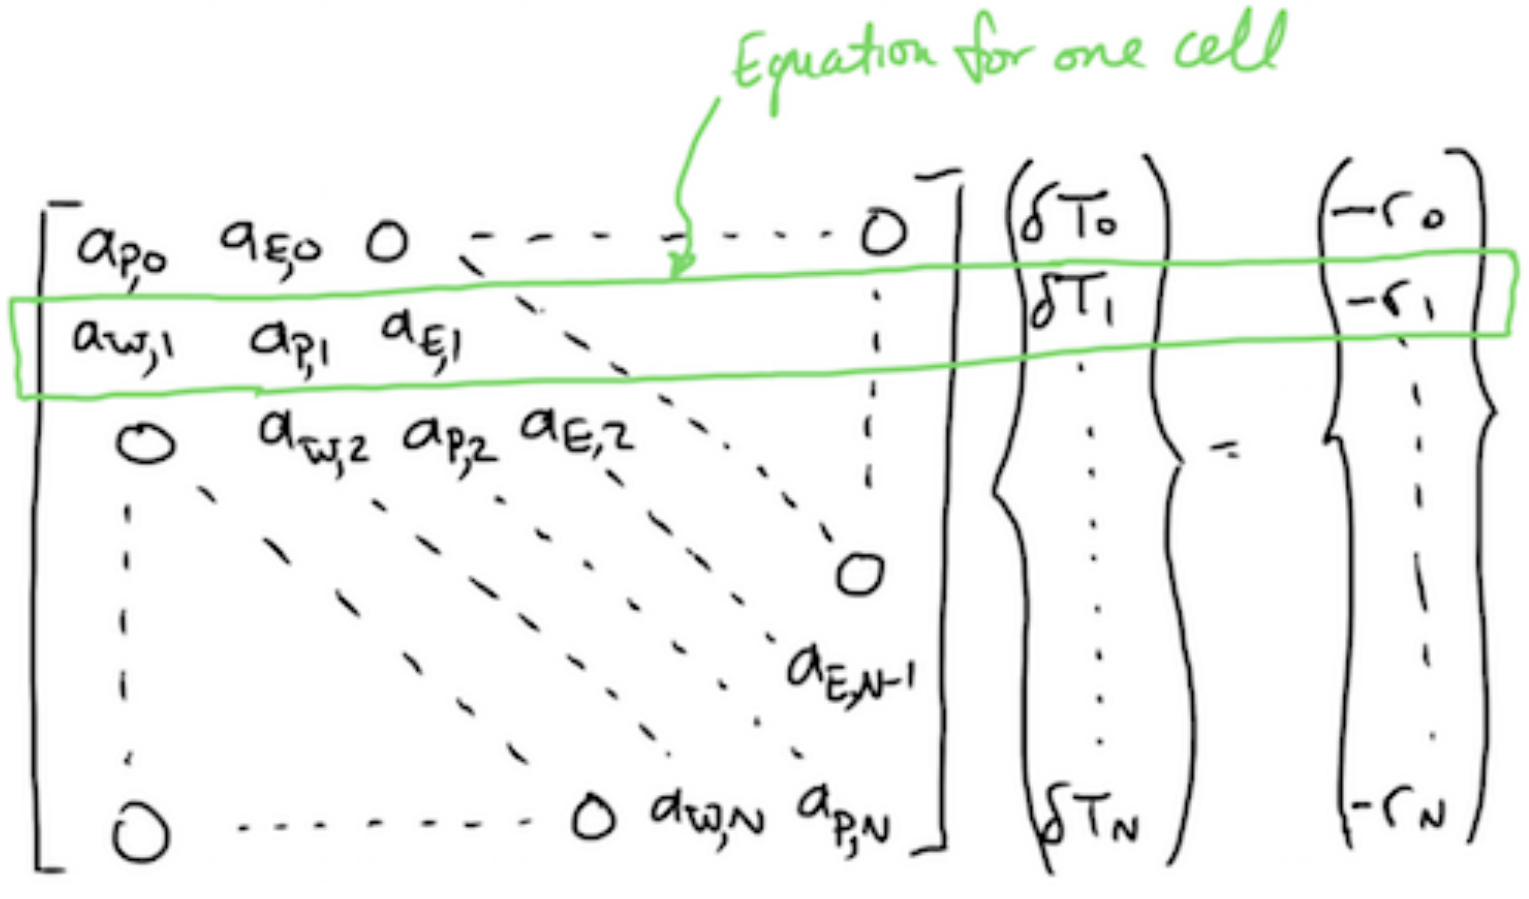
\includegraphics[scale=0.2]{pic/heat1D_tridiagonal.png}
\end{center}
\textbf{Note}: The first and last row only has 2 non zero elements each. This is because these are the left most/right most side and they are
adjacent to the domain boundary. Therefore, special \uline{boundary conditions} are needed to be set. \\
In matrix notation, we are solving:
\begin{equation}
\textbf{A}\textbf{x} = \textbf{b}  
\end{equation}
where \(\textbf{A}\) is the Jacobian matrix, \(\textbf{b} = \textbf{-r}\) is the residual vector, \(\textbf{x} = \delta \textbf{T}\)
is the solution correction. At each current iteration \(i\), the solution is updated according to:
\begin{equation}
\textbf{T} = \textbf{T}_i + \delta \textbf{T}i
\end{equation}
\subsection{Source Terms}
\label{sec:orgfadf074}
Our source term can have many forms, depending on the type of heat source. We will assume \emph{external convection}
and \emph{radiation exchange}:
\begin{itemize}
\item For external convection:
\begin{equation}
\frac{S_{conv,P}}{V_P} = -hA_0(T_P-T_{\infty,c})
\end{equation}
where:
\begin{itemize}
\item \(h\) is the convective coefficient.
\item \(A_0\) is external surface area of the cell \(P\).
\item \(T_P\) is temperature at the centroid of cell \(P\).
\item \(T_{\infty,c}\) is the ambient temperature for the convection process.
\end{itemize}
\item For radiation exchange:
\begin{equation}
\frac{S_{rad}}{V_P} = -\epsilon \sigma A_0(T_P^4 - T_{\infty,r}^4)
\end{equation}
where:
\begin{itemize}
\item \(\epsilon\) is the surface emissivity.
\item \(\sigma\) is the Stefan-Boltzmann constant.
\item \(T_{\infty,r}\) is the surrounding temperature for radiation exchange.
\end{itemize}
\end{itemize}
\subsection{Discussion of Discretization Procedure}
\label{sec:org8f65d60}
\subsubsection{Temperature Profile Assumptions}
\label{sec:org449a010}
When computing the diffusive fluxes through the faces, we assumed a \textbf{piecewise-linear profile} for the temperature.
This ensures that the derivatives are defined at the integration points and provides consistency for flux
at control-volume faces. For the source term, \textbf{piece-wise constant profile} is used, implying a single value of the source
term in each cell. Note that for piece-wise constant profile, the derivatives are not defined at integration points, due to
jump discontinuity. So if fluxes will be inconsistent if piecewise-constant profile is used for temperature.
\begin{center}
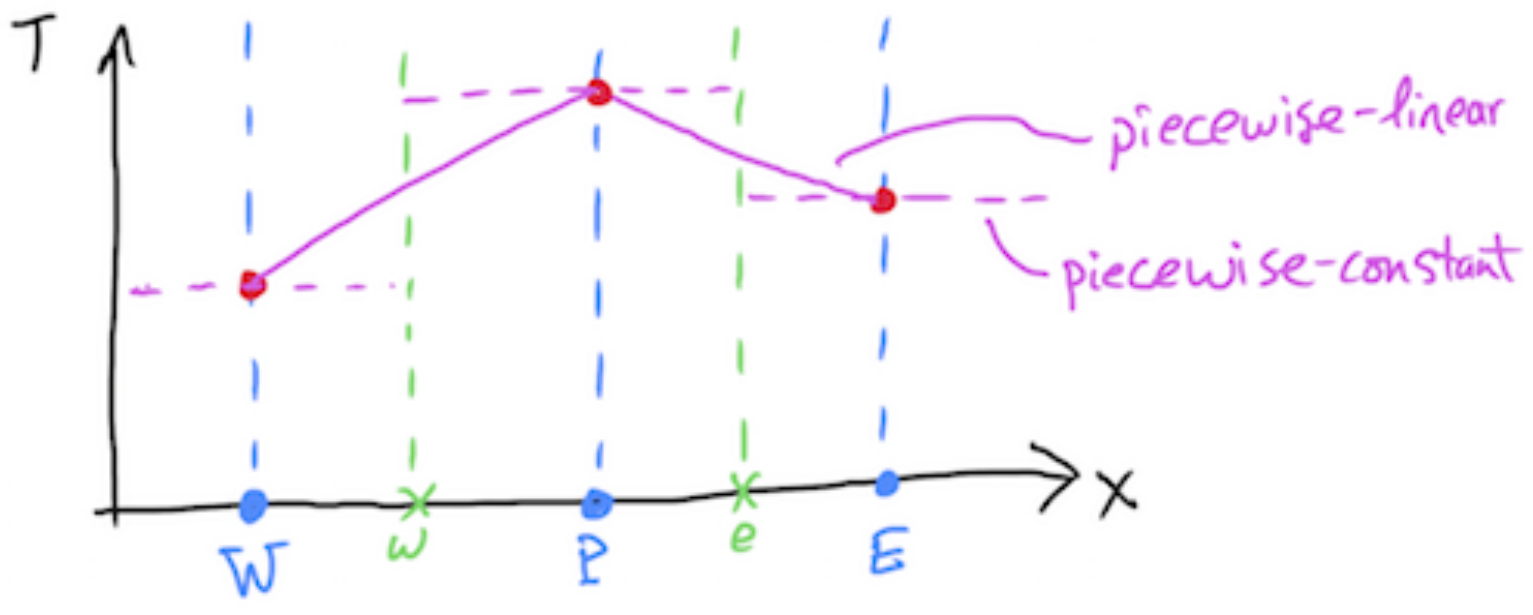
\includegraphics[scale=0.2]{pic/heat1D_profilePW.png}
\end{center}
\subsubsection{Implementation of Linearization}
\label{sec:orgb242044}
In Patakar's method, the solution of the linear system \textbf{is} the solution for the variables at the control volume center.\\
In our method, the solution of the linear system is the \textbf{correction} to apply to the previous iteration of the solution. \\
The correction method is preferred because:
\begin{itemize}
\item at convergence, the solution for the correction goes to zero \(\rightarrow\) zero a good initial guess for the linear solver.
\item linear system involves the residual vector. In Patankar's, there are more work to calculate the residual vector.
\end{itemize}
\subsubsection{Properties of the Discrete Algebraic Equations}
\label{sec:orgbd9a34d}
Recall our algebraic equation for the linear system
\begin{equation}
a_P\delta T_P + a_W\delta T_W + a_E \delta T_E = -r_P 
\end{equation}
In Rule 2, we require that \(a_P > 0\) and \(a_W, a_E < 0\). The reason for this is if we consider the case with no source,
and the solution converge, \(r_P \rightarrow 0\):
\begin{equation}
a_P\delta T_P = -a_W\delta T_W - a_E \delta T_E  
\end{equation}
Now, suppose both \(T_P\) and \(T_E\) are pertubed.  If either of these temperatures were to rise, then \(T_P\) would also rise.
Similarly, if either temperatures were to drop, \(T_P\) should also drop. Therefore, to ensure correct physical effect, if
\(a_P > 0\) then \(a_W, a_E > 0\).\\
Consider the two cells (\(P\) and \(E\)) below:
\begin{center}
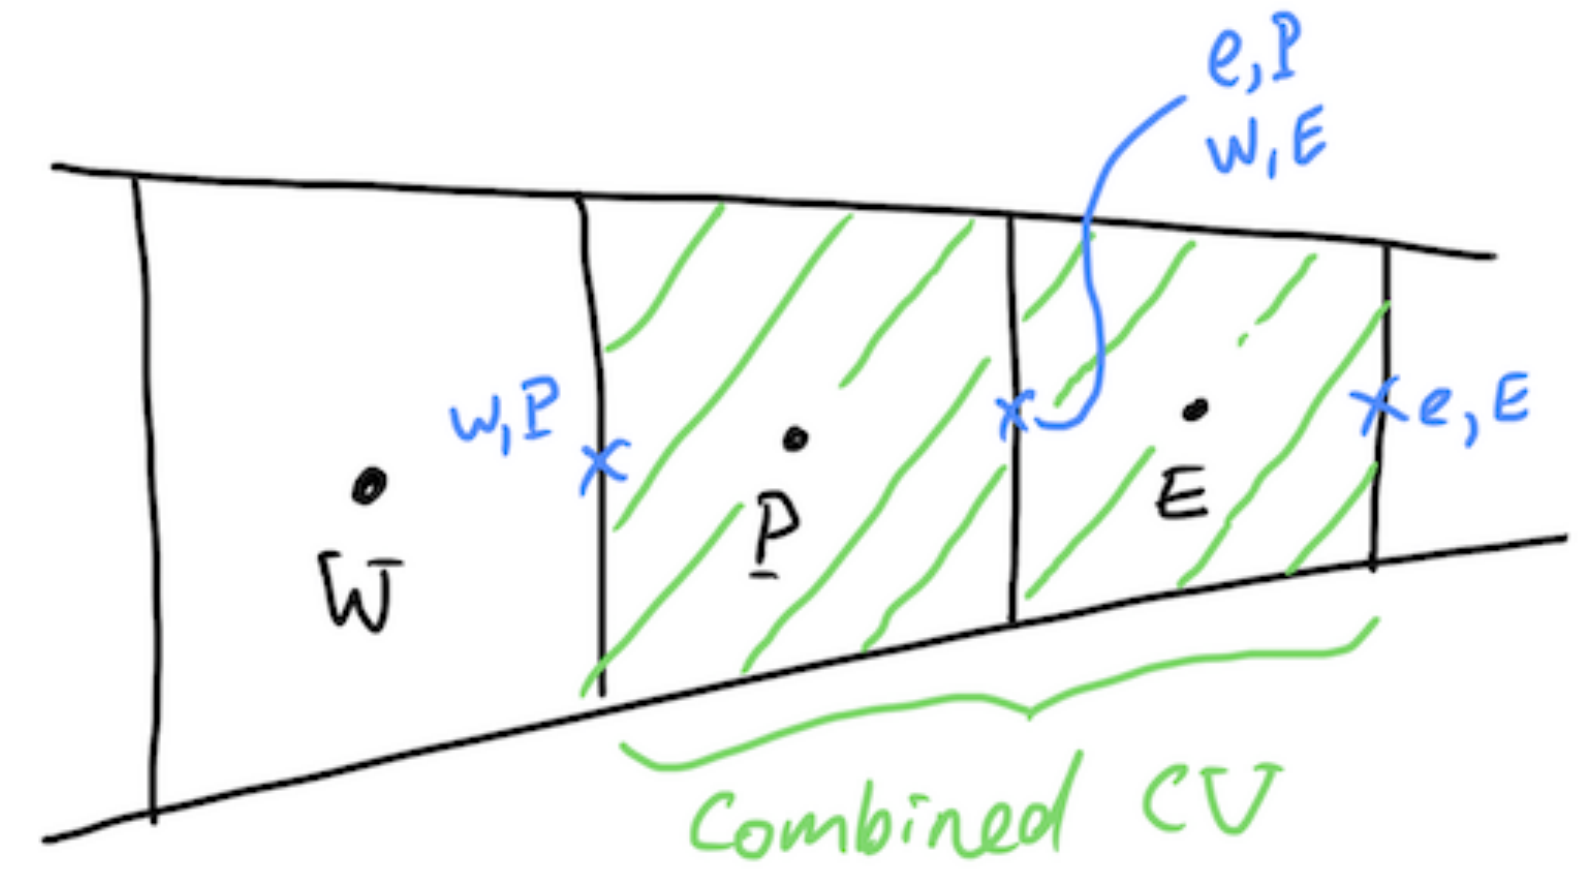
\includegraphics[scale=0.2]{pic/heat1D_cell_combined.png}
\end{center}
At convergence, \(r_P = 0\), the equation for the control volume \(P\) is:
\begin{equation}
F_{e,P}^d - F_{w,P}^d - S_PV_P = 0
\end{equation}
For the control volume \(E\):
\begin{equation}
F_{e,E}^d - F_{w,E}^d - S_EV_E = 0
\end{equation}
Adding these equations together gives:
\begin{equation}
F_{e,P}^d - F_{w,P}^d +  F_{e,E}^d - F_{w,E}^d- S_PV_P - S_EV_E = 0
\end{equation}
Note that \(F_{e,P}^d = F_{w,E}^d\) by continuity, i.e. the flux at cell \(P\) going eastward should be the same flux going
from westward at cell \(E\). If these are not equal, then it implies that there is a fictuous force at the face, which is
not reasonable. Therefore, our algebraic equation for control volume \(P\) and \(E\) becomes:
\begin{equation}
 F_{e,E}^d - F_{w,P}^d - S_PV_P - S_EV_E = 0
\end{equation}
The above equation demonstrates integral conservation: a balance of the total source term within the combined control volume with
the net diffusive flux from that same control volume. In addition, recall the definition of the diffusive flux:
\begin{align}
F_{e,P}^d &= -k \frac{T_E-T_P}{\Delta x_{PE}} A_{e,P}\\
F_{w,E}^d &= -k \frac{T_E-T_P}{\Delta x_{PE}} A_{w,E}
\end{align}
From the gemeotry of the grid, \(A_{e,P} = A_{w,E}\); therefore, it is in fact the two-point finite difference estimation of the
derivative that cause the fluxes to be equal. This is also due to the piecewise-linear profile that we assume. If we assume a
\textbf{parabolic profile} instead, there is no guarantee that the fluxes would be equal. Instead, we would have:
\begin{align}
F_{e,P}^d &= f(T_W, T_P, T_E)\\
F_{w,E}^d &= f(T_P, T_E, T_{EE})
\end{align}
This means that the flux through the common face depends on different temperature, so we cannot be sure that the derivative from either
side is consistent. 
\begin{center}
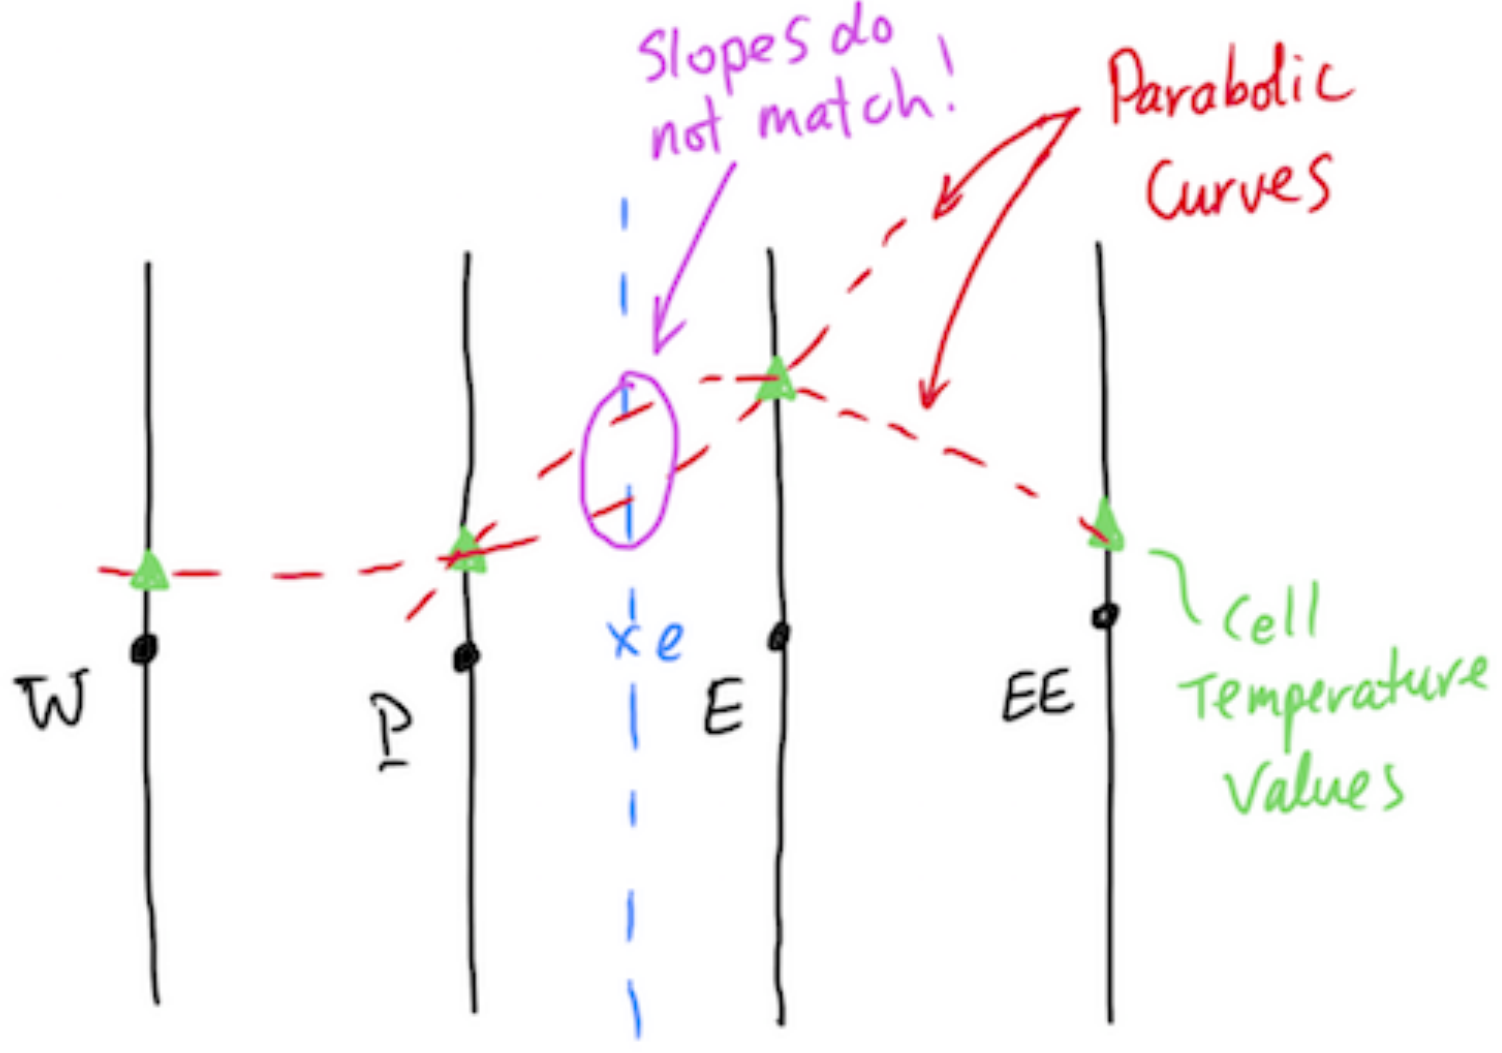
\includegraphics[scale=0.2]{pic/heat1D_profilePARABOLIC.png}
\end{center}
\subsection{Implemenation: \href{1D\_heat\_diffusion\_steady.py}{Python Code}}
\label{sec:orga28fc2f}
\lstinputlisting[language=Python]{1D_heat_diffusion_steady.py}
\end{document}